\chapter{Specifikacija programske potpore}
		
	\section{Funkcionalni zahtjevi}			
			
			\noindent \textbf{Dionici:}
			
			\begin{packed_enum}
				
				\item Pacijent
				\item Djelatnik	
				\begin{packed_item}
					\item Liječnik
					\item Administrator
				\end{packed_item}
				\item Razvojni tim
				
			\end{packed_enum}
			
			Pacijenti i djelatnici zajedničkim imenom su korisnici.
			
			
			\noindent \textbf{Aktori i njihovi funkcionalni zahtjevi:}
			
			
			\begin{packed_enum}
				\item  \underbar{Neregistrirani korisnik (inicijator) može:}
				\begin{packed_enum}
					\item registrirati se u sustav, unijeti potrebne podatke(ime, prezime, e-mail adresu, MBO, broj telefona, lozinku)
				\end{packed_enum}
			
				\item  \underbar{Neprijavljeni korisnik (inicijator) može:}
				\begin{packed_enum}
					\item prijaviti se u sustav koristeći svoju e-mail adresu i lozinku
					\item promijeniti zaboravljenu lozinku
				\end{packed_enum}
				
				\item  \underbar{Pacijent-\textit{prijavljeni korisnik} (inicijator) može:}
				\begin{packed_enum}
					\item prikazati i mijenjati svoje osobne podatke i lozinku
					\item prikazati svoje terapije (tip rehabilitacije, liječnika koji ga je uputio na rehabilitaciju, referencu na prošlu terapiju i status)
					\item prikazati svoje termine (vrijeme termina, prostoriju, tip rehabilitacije, liječnika, napomene i ishod termina) 
					\item filtrirati svoje termine
					\item prikazati nalaz (detalji i komentari) s odrađenog termina
					\item naručiti se na terapiju, unijeti tip rehabilitacije, liječnika koji ga je uputio na terapiju, opis oboljenja i zahtijevani postupak liječenja
					\item odabrati termin za neku od aktivnih terapija
					\item promijeniti termin????
				\end{packed_enum}
				
				\item  \underbar{Djelatnik-\textit{prijavljeni korisnik} (inicijator) može:}
				\begin{packed_enum}
					\item prikazati i mijenjati svoje osobne podatke i lozinku
					\item vidjeti popis svih pacijenata (ime, prezime, MBO, e-mail adresa, broj telefona)
					\item prikazati termine pojedinog pacijenta i prikazati evidenciju termina pojedinog pacijenta
					\item evidentirati dolazak pacijenta na termin, dodati komentar o odrađenom terminu i vidjeti informacije o terapiji
					\item promijeniti i otkazati zakazani termin
				\end{packed_enum}
				\item  \underbar{Administrator - \textit{prijavljeni korisnik} (inicijator)  može:}
				\begin{packed_enum}
					
					\item vidjeti popis svih djelatnika (ime, prezime, OIB, e-mail adresa)
					\item urediti podatke djelatnika
					\item ukloniti djelatnika
					\item dodati/registrirati novog djelatnika (ime, prezime, e-mail adresa, OIB, lozinka)
					\item mijenjati raspoloživost soba i opreme
					\item dodavati opremu i sobe
					
				\end{packed_enum}
				
				\item  \underbar{Baza podataka (sudionik):}
				\begin{packed_enum}
					
					\item pohranjuje podatke i ovlasti korisnika
					\item pohranjuje podatke o opremi i prostorijama
					\item pohranjuje podatke o terapijama i terminima
					
				\end{packed_enum}
			\end{packed_enum}
			
			\eject 
			
			
				
			\subsection{Obrasci uporabe}
				
				
				\subsubsection{Opis obrazaca uporabe}
					

					\noindent \underbar{\textbf{UC1 - Prijava u sustav}}
					\begin{packed_item}
	
						\item \textbf{Glavni sudionik: }Korisnik
						\item  \textbf{Cilj: } Prijaviti se u sustav
						\item  \textbf{Sudionici: } Baza podataka
						\item  \textbf{Preduvjet: } Korisnik je registriran u sustav
						\item  \textbf{Opis osnovnog tijeka: }
						
						\item[] \begin{packed_enum}
	
							\item Korisnik unosi svoju e-mail adresu i lozinku
							\item Provjera ispravnosti podataka
							\item Prikaz početne stranice ovisno o korisniku
						\end{packed_enum}
						
						\item  \textbf{Opis mogućih odstupanja:}
						
						\item[] \begin{packed_item}
							\item[1.a] Korisnik je zaboravio lozinku
							\item[] \begin{packed_enum}
								
								\item Korisnik odabire opciju "Zaboravili ste lozinku?"
								\item Korisnik unosi e-mail adresu
								\item Nakon potvrde korisniku se šalje e-mail s novom lozinkom
								\item Korisnik ponovno unosi podatke
								
							\end{packed_enum}
							\item[2.a] Neispravna e-mail adresa ili lozinka
							\item[] \begin{packed_enum}
								
								\item obavijest o neispravnosti unesenih podataka
								
							\end{packed_enum}
							
						\end{packed_item}
					\end{packed_item}
				
				\noindent \underbar{\textbf{UC2 - Registracija}}
				\begin{packed_item}
					
					\item \textbf{Glavni sudionik: }Neregistrirani korisnik
					\item  \textbf{Cilj: }Registrirati se u sustav
					\item  \textbf{Sudionici: }Baza podataka
					\item  \textbf{Preduvjet: } -  
					\item  \textbf{Opis osnovnog tijeka: }
					
					\item[] \begin{packed_enum}
						
						\item Korisnik unosi svoje podatke (ime, prezime, e-mail adresu, MBO, lozinka)
						\item Provjera ispravnosti podataka verifikacijom iz baze podataka sustava zdravstvene zaštite
						\item Slanje maila za verifikaciju e-mail adrese
						\item Korisnik klikom na link verificira svoju e-mail adresu
						\item Prikaz stranice za prijavu u sustav
					\end{packed_enum}
					
					\item  \textbf{Opis mogućih odstupanja:}
					
					\item[] \begin{packed_item}
						
						\item[2.a] Korisnik ne postoji u sustavu zdravstvene zaštite
						\item[] \begin{packed_enum}
							
							\item Sustav obavještava korisnika o neispravnosti podataka
							\item Korisnik mijenja podatke ili odustaje od registracije
							
						\end{packed_enum}
						
					\end{packed_item}
				\end{packed_item}
				
				\noindent \underbar{\textbf{UC3 - pregled osobnih podataka}}
				\begin{packed_item}
					
					\item \textbf{Glavni sudionik: }Korisnik
					\item  \textbf{Cilj: }Pregledati osobne podatke 
					\item  \textbf{Sudionici: }Baza podataka
					\item  \textbf{Preduvjet: }Korisnik mora biti prijavljen u sustav
					\item  \textbf{Opis osnovnog tijeka: }
					
					\item[] \begin{packed_enum}
						
						\item Korisnik odabire opciju "Profil"
						\item Sustav prikazuje korisnikove osobne podatke 
					\end{packed_enum}
					
				\end{packed_item}
				\noindent \underbar{\textbf{UC4 - Promjena broja telefona}}
				\begin{packed_item}
					
					\item \textbf{Glavni sudionik: }Korisnik
					\item  \textbf{Cilj: }Promijeniti broj telefona
					\item  \textbf{Sudionici: }Baza podataka
					\item  \textbf{Preduvjet: }Korisnik mora biti prijavljen u sustav
					\item  \textbf{Opis osnovnog tijeka: }
					
					\item[] \begin{packed_enum}
						
						\item Korisnik odabire opciju "Promijeni broj telefona"  
						\item Korisnik unosi/mijenja broj telefona
						\item Korisnik odabire opciju "Spremi"
						\item Povratak na prikaz osobnih podataka
					\end{packed_enum}
				\end{packed_item}
				
				\noindent \underbar{\textbf{UC5 - Promjena lozinke}}
				\begin{packed_item}
					
					\item \textbf{Glavni sudionik: }Korisnik
					\item  \textbf{Cilj: }Promijeniti lozinku
					\item  \textbf{Sudionici: }Baza podataka
					\item  \textbf{Preduvjet: }Korisnik je prijavljen u sustav
					\item  \textbf{Opis osnovnog tijeka: }
					
					\item[] \begin{packed_enum}
						
						\item Korisnik odabire opciju "Promijeni lozinku"
						\item Korisnik unosi staru lozinku
						\item Korisnik unosi novu lozinku
						\item Korisnik potvrđuje novu lozinku
						\item Povratak na prikaz podataka
					\end{packed_enum}
					
					\item  \textbf{Opis mogućih odstupanja:}
					
					\item[] \begin{packed_item}
						
						\item[2.a] korisnik unosi neispravnu staru lozinku
						\item[] \begin{packed_enum}
							
							\item Sustav upozorava korisnika o neispravnosti lozinke
							\item Korisnik ponovno mijenja lozinku ili odustaje od promjene
							
						\end{packed_enum}
						\item[3.a] Nova lozinka je jednaka staroj
						\item[]\begin{packed_enum}
							
							\item Sustav upozorava korisnika da su mu lozinke iste
							\item Korisnik mijenja novu lozinku ili odustaje od promjene
							
						\end{packed_enum}
						
					\end{packed_item}
				\end{packed_item}
				
				\noindent \underbar{\textbf{UC6 - Kreiranje terapije(\ref{fig:sekvencijski_dijagram_1})}}
				\begin{packed_item}
					
					\item \textbf{Glavni sudionik: }Pacijent
					\item  \textbf{Cilj: }Kreiranje procesa terapije
					\item  \textbf{Sudionici: }Baza podataka
					\item  \textbf{Preduvjet: }Pacijent je prijavljen u sustav
					\item  \textbf{Opis osnovnog tijeka: }
					
					\item[] \begin{packed_enum}
						
						\item Pacijent odabire opciju "Nova terapija"
						\item Otvara se stranica za kreiranje terapije
						\item Pacijent unosi ime i prezime liječnika, opis oboljenja i zahtijevani postupak liječenja, te odabire vrstu terapije
						\item Pacijent odabire opciju "Potvrdi"
						\item Provjera ispravnosti podataka u imeniku liječnika
						\item Prikaz stranice za odabir termina
					\end{packed_enum}
					
					\item  \textbf{Opis mogućih odstupanja:}
					
					\item[] \begin{packed_item}
						
						\item[3.a] Liječnik ne postoji u imeniku liječnika
						\item[] \begin{packed_enum}
							
							\item Sustav obavještava pacijenta o neispravnim podacima(ime i prezime liječnika)
							\item Pacijent mijenja podatke ili odustaje od kreiranja terapije
							
						\end{packed_enum}
												
					\end{packed_item}
				\end{packed_item}
				\noindent \underbar{\textbf{UC7 - Odabir termina}}
				\begin{packed_item}
					
					\item \textbf{Glavni sudionik: }Pacijent
					\item  \textbf{Cilj: }Poslati zahtjev za željenim terminom
					\item  \textbf{Sudionici: }Baza podataka
					\item  \textbf{Preduvjet: }Pacijent je prijavljen u sustav
					\item  \textbf{Opis osnovnog tijeka: }
					
					\item[] \begin{packed_enum}
						
						\item Pacijent odabire terapiju za koju se prijavljuje na termin
						\item Otvara se stranica s popisom termina te terapije i gumbom za novu terapiju
						\item Pacijent odabire opciju "Novi termin"
						\item Otvara se stranica za prijavu termina
						\item Pacijent unosi datum i vrijeme
						\item Pacijent šalje zahtjev klikom na "Potvrdi"
						\item Spremanje podataka u bazu i slanje maila s podatcima o terminu
						
					\end{packed_enum}
					
					\item  \textbf{Opis mogućih odstupanja:}
					
					\item[] \begin{packed_item}
						\item[5.a] Pacijentu ne odgovara niti jedan termin
						\item[] \begin{packed_enum}
							
							\item Pacijent odustaje od prijave na termin
							
						\end{packed_enum}
						
						\item[7.a] Termin koji je pacijent odabrao se u međuvremenu popunio
						\item[] \begin{packed_enum}
							
							\item Sustav ne sprema podatke u bazu i obaviještava korisnika o zauzetom terminu
							\item Pacijent mijenja podatke ili odustaje od prijave termina
							
						\end{packed_enum}
						
					\end{packed_item}
				\end{packed_item}
				
			
				
				\noindent \underbar{\textbf{UC8 - Prikaz nalaza termina}}
				\begin{packed_item}
					
					\item \textbf{Glavni sudionik: }Pacijent
					\item  \textbf{Cilj: }Pacijent vidi svoje termine
					\item  \textbf{Sudionici: }Baza podataka
					\item  \textbf{Preduvjet: }Prijavljen u sustav, postoje prošli termini
					\item  \textbf{Opis osnovnog tijeka: }
					
					\item[] \begin{packed_enum}
						
						\item Pacijent odabire opciju prikaži nalaz
						\item Otvara se skočni prozor s informacijama i komentarom liječnika (nalazom)
						\item Pacijent odabire opciju zatvori u skočnom prozoru
					\end{packed_enum}
				\end{packed_item}
				
				\noindent \underbar{\textbf{UC9 - Prikaz pacijenta}}
				\begin{packed_item}
					
					\item \textbf{Glavni sudionik: }Djelatnik
					\item  \textbf{Cilj: }Prikazati termine pojedinog pacijenta 
					\item  \textbf{Sudionici: }Baza podataka
					\item  \textbf{Preduvjet: }Djelatnik je prijavljen u sustav
				
					\item  \textbf{Opis osnovnog tijeka: }
					
					\item[] \begin{packed_enum}
						
						\item Djelatnik pretražuje pacijenta upisom imena i prezimena u tražilicu
						\item Djelatnik odabire opciju "Prikaži termine" pored željenog pacijenta
						\item Sustav otvara tablicu termina odabranog pacijenta
						\item Djelatnik otvara 
						\item Djelatnik evidentira(UC10)/prikazuje evidenciju(UC8)
						\item Djelatnik odabire opciju povratka na popis pacijenata
					\end{packed_enum}
					
					\item  \textbf{Opis mogućih odstupanja:}
					
					\item[] \begin{packed_item}
						
						\item[1.a] Upisani pacijent ne postoji u sustavu
						\item[] \begin{packed_enum}
							\item Prikaz teksta o ne postojanju pacijenta
							\item Djelatnik mijenja upisano ime i prezime ili odustaje od pretraživanja
							
						\end{packed_enum}
						
					\end{packed_item}
					\item[] \begin{packed_item}
						
						\item[3.a] Odabrani pacijent još nije bio ni na jednoj terapiji
						\item[] \begin{packed_enum}
							\item Prikaz teksta o ne postojanju termina za odabranog pacijenta
							\item Djelatnik odabire opciju povratka na popis pacijenata
											 							
						\end{packed_enum}
						
					\end{packed_item}
				\end{packed_item}
				
				\noindent \underbar{\textbf{UC10 - Evidencija dolaska(\ref{fig:sekvencijski_dijagram_2})}}
				\begin{packed_item}
					
					\item \textbf{Glavni sudionik: }Djelatnik
					\item  \textbf{Cilj: }Evidentirati dolazak pacijenta na termin 
					\item  \textbf{Sudionici: }Baza podataka
					\item  \textbf{Preduvjet: }
					\item[] \begin{packed_enum}
						
						\item[-] Djelatnik je prijavljen u sustav
						\item[-] Pacijent mora imati termin koji nije evidentiran
					\end{packed_enum}
					\item  \textbf{Opis osnovnog tijeka: }
					
					\item[] \begin{packed_enum}
						\item Djelatnik odabire termin koji će evidentirati
						\item Otvara se stranica termina
						\item Djelatnik odabire opciju "Evidentiraj"
						\item Otvara se obrazac za evidenciju dolaska na termin
						\item Djelatnik evidentira dolazak odabirom jedne od tri ponuđene opcije(nije došao, došao je, otkazano)
						\item Djelatnik unosi komentar o odrađenom terminu i napredku
						\item Djelatnik predaje evidenciju
						\item Povratak na stranicu termina
					\end{packed_enum}
					
					\item  \textbf{Opis mogućih odstupanja:}
					
					\item[] \begin{packed_item}
						
						\item[3.a] Djelatnik odustaje od evidentiranja termina
						\item[] \begin{packed_enum}
							\item Djelatnik odabire opciju povratka na popis termina odabranog pacijenta
							
						\end{packed_enum}
					\end{packed_item}
				\end{packed_item}
				
					
				
				\noindent \underbar{\textbf{UC11 - Registracija djelatnika}}
				\begin{packed_item}
					
					\item \textbf{Glavni sudionik: }Administrator
					\item  \textbf{Cilj: }Registrirati novog djelatnika
					\item  \textbf{Sudionici: }Baza podataka
					\item  \textbf{Preduvjet: }
					\item[] \begin{packed_enum}
						
						\item[-] Djelatnik je prijavljen u sustav
						\item[-] Djelatnik ima ovlasti administratora
					\end{packed_enum}
					\item  \textbf{Opis osnovnog tijeka: }
					
					\item[] \begin{packed_enum}
						\item Djelatnik odaibre opciju "Dodaj djelatnika"
						\item Prikazuje se stranica za registraciju novog djelatnika
						\item Administrator unosi podatke o djelatniku(ime, prezime, OIB, e-mail adresu i inicijalnu lozinku)
						\item Administrator odabire opciju "Dodaj račun"
						\item Podatci se unose u bazu podataka
					\end{packed_enum}
					
					\item  \textbf{Opis mogućih odstupanja:}
					
					\item[] \begin{packed_item}
						
						\item[3.a] Podatci ne zadovoljavaju željeni format
						\item[] \begin{packed_enum}
							\item Sustav upozorava administratora o neispravnom formatu podataka
							\item Administrator mijenja podatke ili odustaje od registracije djelatnika							
						\end{packed_enum}
					\end{packed_item}
				\end{packed_item}
				
				\noindent \underbar{\textbf{UC12 - Uređivanje podataka djelatnika}}
				\begin{packed_item}
					
					\item \textbf{Glavni sudionik: }Administrator
					\item  \textbf{Cilj: }Promijeniti podatke djelatnika
					\item  \textbf{Sudionici: }Baza podataka
					\item  \textbf{Preduvjet: }
					\item[] \begin{packed_enum}
						
						\item[-] Djelatnik je prijavljen u sustav
						\item[-] Djelatnik ima ovlasti administratora
						\item[-] Postoji barem jedan liječnik/djelatnik
					\end{packed_enum}
					\item  \textbf{Opis osnovnog tijeka: }
					
					\item[] \begin{packed_enum}
						\item Administrator odabire opciju "Uredi" pokraj imena djelatnika
						\item Prikazuje se stranica s podacima odabranog djelatnika
						\item Administrator mijenja podatke o djelatniku(ime, prezime, OIB, e-mail adresu)
						\item Administrator odabire opciju "Spremi"
						\item Podatci se mijenjaju u bazi podataka
						\item Prikazuje se popis djelatnika
					\end{packed_enum}
					
					\item  \textbf{Opis mogućih odstupanja:}
					
					\item[] \begin{packed_item}
						
						\item[3.a] Podatci ne zadovoljavaju željeni format
						\item[] \begin{packed_enum}
							\item Sustav upozorava administratora o neispravnom formatu podataka
							\item Administrator mijenja podatke ili odustaje od promjene podataka							
						\end{packed_enum}
						
						\item[4.a] Administrator ne želi promijeniti podatke 
						\item[] \begin{packed_enum}
							\item Administrator odabire opciju "Odustani"
							\item Podatci se ne mijenjaju u bazi podataka
							\item Prikazuje se popis djelatnika							
						\end{packed_enum}
					\end{packed_item}
				\end{packed_item}
				
				
				\noindent \underbar{\textbf{UC13 - Promjena ovlasti djelatnika}}
				\begin{packed_item}
					
					\item \textbf{Glavni sudionik: }Administrator
					\item  \textbf{Cilj: }Promijeniti ovlasti djelatnika
					\item  \textbf{Sudionici: }Baza podataka
					\item  \textbf{Preduvjet: }
					\item[] \begin{packed_enum}
						
						\item[-] Djelatnik je prijavljen u sustav
						\item[-] Djelatnik ima ovlasti administratora
						\item[-] Postoji barem jedan liječnik/djelatnik
					\end{packed_enum}
					\item  \textbf{Opis osnovnog tijeka: }
					
					\item[] \begin{packed_enum}
						\item Administrator odabire opciju "Uredi" pokraj imena djelatnika
						\item Prikazuje se stranica s podacima odabranog djelatnika
						\item Administrator odabire opciju "Promijeni ovlasti"
						\item Otvara se skočni prozor 
						\item Administrator pridjeljuje/uklanja administratorske ovlasti djelatnika
						\item Administrator odabire opciju "Spremi"
						\item Otvara se skočni prozor s upozorenjem i zahtjevom za unos lozinke administratora
						\item Administrator unosi lozinku
						\item Administrator odabire opcije "potvrdi"
						\item Sustav potvrđuje lozinku i sprema promjene u bazu podataka
						\item Vraća se na podatke o djelatniku
					\end{packed_enum}
					
					\item  \textbf{Opis mogućih odstupanja:}
					
					\item[] \begin{packed_item}
						
						\item[10.a] Administrator je unio neispravnu lozinku
						\item[] \begin{packed_enum}
							\item Sustav upozorava administratora o unosu neispravne lozinke 
							\item Administrator ponovno unosi lozinku ili odustaje od promjene ovlasti						
						\end{packed_enum}
				\end{packed_item}
			\end{packed_item}
				
				\noindent \underbar{\textbf{UC14 - Uklanjanje djelatnika}}
				\begin{packed_item}
					
					\item \textbf{Glavni sudionik: }Administrator
					\item  \textbf{Cilj: }Ukloniti djelatnika
					\item  \textbf{Sudionici: }Baza podataka
					\item  \textbf{Preduvjet: }
					\item[] \begin{packed_enum}
						
						\item[-] Djelatnik je prijavljen u sustav
						\item[-] Djelatnik ima ovlasti administratora
						\item[-] Postoji barem jedan liječnik/djelatnik
					\end{packed_enum}
					\item  \textbf{Opis osnovnog tijeka: }
					
					\item[] \begin{packed_enum}
						\item Administrator odabire opciju "Ukloni" pokraj imena djelatnika
						\item Otvara se skočni prozor s upozorenjem i zahtjevom za unos lozinke administratora
						\item Administrator unosi lozinku
						\item Administrator odabire opciju "Potvrdi"
						\item Sustav potvrđuje lozinku
						\item U bazi podataka se mijenja vrijednost atributa jeAktivan odabranog djelatnika
						\item prikazuje se popis djelatnika bez upravo uklonjenog djelatnika
					\end{packed_enum}
					
					\item  \textbf{Opis mogućih odstupanja:}
					
					\item[] \begin{packed_item}
						
						\item[5.a] Administrator je unio neispravnu lozinku
						\item[] \begin{packed_enum}
							\item Sustav upozorava administratora o unosu neispravne lozinke 
							\item Administrator ponovno unosi lozinku ili odustaje od uklanjanja djelatnika					
						\end{packed_enum}
					\end{packed_item}
				\end{packed_item}
					
					
					\noindent \underbar{\textbf{UC15 - Unos opreme}}
					\begin{packed_item}
						
						\item \textbf{Glavni sudionik: }Administrator
						\item  \textbf{Cilj: }Unos opreme
							\item  \textbf{Sudionici: }Baza podataka
							\item  \textbf{Preduvjet: }
							\item[] \begin{packed_enum}
								
								\item[-] Djelatnik je prijavljen u sustav
								\item[-] Djelatnik ima ovlasti administratora
							\end{packed_enum}
							\item  \textbf{Opis osnovnog tijeka: }
							
							\item[] \begin{packed_enum}
								\item Administrator odabire opciju "Inventar"
								\item Otvara se stranica s popisom opreme
								\item Administrator odabire opciju "Dodaj opremu"
								\item Otvara se skočni prozor s prostorom za unos podataka o opremi
								\item Unosi podatke o opremi (ime i opis)
								\item Odabire prostoriju u kojoj će se oprema nalaziti
								\item Administrator odabire opciju "Spremi"
								\item Podatci se spremaju u bazu podataka i generira se jedinstveni identifikator opreme
								\item Prikazuje se stranica s popisom opreme
							\end{packed_enum}
							
							\item  \textbf{Opis mogućih odstupanja:}
							
							\item[] \begin{packed_item}
								
								\item[6.a] Administrator želi odustati od unosa opreme 
								\item[] \begin{packed_enum}
									\item 	Administrator odabire opciju "odustani"			
								\end{packed_enum}
							\end{packed_item}
						\end{packed_item}
				
				
				\noindent \underbar{\textbf{UC16 - Promjena dostupnosti opreme}}
				\begin{packed_item}
					
					\item \textbf{Glavni sudionik: }Administrator
					\item  \textbf{Cilj: }Promjeniti dostupnost opreme
					\item  \textbf{Sudionici: }Baza podataka
					\item  \textbf{Preduvjet: }
					\item[] \begin{packed_enum}
						
						\item[-] Djelatnik je prijavljen u sustav
						\item[-] Djelatnik ima ovlasti administratora
					\end{packed_enum}
					\item  \textbf{Opis osnovnog tijeka: }
					
					\item[] \begin{packed_enum}
						\item Administrator odabire opciju "Inventar"
						\item Otvara se stranica s popisom opreme
						\item Administrator pretražuje opremu
						\item Administrator mijenja dostupnost opreme odabirom opcije "Dostupno"/"Nedostupno"
						\item Promjena dostupnosti odabrane opreme u bazi podataka
					\end{packed_enum}
					
				\end{packed_item}
				
				\noindent \underbar{\textbf{UC17 - Unos prostorija}}
				\begin{packed_item}
					
					\item \textbf{Glavni sudionik: }Administrator
					\item  \textbf{Cilj: }Unijeti nove prostorije
					\item  \textbf{Sudionici: }Baza podataka
					\item  \textbf{Preduvjet: }
					\item[] \begin{packed_enum}
						
						\item[-] Djelatnik je prijavljen u sustav
						\item[-] Djelatnik ima ovlasti administratora
					\end{packed_enum}
					\item  \textbf{Opis osnovnog tijeka: }
					
					\item[] \begin{packed_enum}
						\item Administrator odabire opciju "Prostorije"
						\item Otvara se stranica s popisom prostorija
						\item Administrator odabire opciju "Dodaj prostoriju"
						\item Prikazuje se skočni prozor s prostorom za unos podataka o prostoriji
						\item Administrator unosi broj i kapacitet prostorije
						\item Administrator odabire opciju "spremi"
						\item Podatci se spremaju u bazu podataka
						\item Prikazuje se stranica s popisom opreme
					\end{packed_enum}
					
					\item  \textbf{Opis mogućih odstupanja:}
					
					\item[] \begin{packed_item}
						
						\item[6.a] Administrator želi odustati od unosa prostorije 
						\item[] \begin{packed_enum}
							\item Administrator odabire opciju "Odustani"
							\end{packed_enum}
					\end{packed_item}
				\end{packed_item}
				
				\noindent \underbar{\textbf{UC18 - Promjena dostupnosti prostorije}}
				\begin{packed_item}
					
					\item \textbf{Glavni sudionik: }Administrator
					\item  \textbf{Cilj: }Promjeniti dostupnost prostorije
					\item  \textbf{Sudionici: }Baza podataka
					\item  \textbf{Preduvjet: }
					\item[] \begin{packed_enum}
						
						\item[-] Djelatnik je prijavljen u sustav
						\item[-] Djelatnik ima ovlasti administratora
					\end{packed_enum}
					\item  \textbf{Opis osnovnog tijeka: }
					
					\item[] \begin{packed_enum}
						\item Administrator odabire opciju "Prostorije"
						\item Otvara se stranica s popisom prostorija
						\item Administrator pretražuje prostorije
						\item Administrator mijenja dostupnost željene prostorije odabirom opcije "Dostupno"/"Nedostupno" koja se nalazi pored podataka o prostoriji
						\item Promjena dostupnosti odabrane prostorije u bazi podataka
					\end{packed_enum}
					
				\end{packed_item}
				
				\noindent \underbar{\textbf{UC19 - Obavijest o promjeni termina}}
				\begin{packed_item}
					
					\item \textbf{Glavni sudionik: }Administrator
					\item  \textbf{Cilj: }Unijeti podatke o novom terminu i obavijestiti pacijenta o tome putem e-maila 
					\item  \textbf{Sudionici: }Baza podataka
					\item  \textbf{Preduvjet: }
					\item[] \begin{packed_enum}
						
						\item[-] Djelatnik je prijavljen u sustav
						\item[-] Djelatnik ima ovlasti administratora
					\end{packed_enum}
					\item  \textbf{Opis osnovnog tijeka: }
					
					\item[] \begin{packed_enum}
						\item Administrator odabire opciju "Promjena termina"
						\item Otvara se stranica s prostorom za podatke o pacijentu i terminu
						\item Administrator pretražuje i odabire pacijenta
						\item Prikazuju se termini odabranog pacijenta koji još nisu evidentirani
						\item Administrator odabire termin koji želi promijeniti
						\item Administrator unosi željene podatke o novom terminu
						\item Prikaz mogućih termina sa željenim podacima
						\item Odabir termina
						\item Administrator opcionalno dodaje komentar
						\item Administrator odabire opciju "Pošalji"
						\item Podaci o terminu se spremaju u bazu podataka
						\item Odabranom pacijentu se šalje e-mail o promjenama i informacijama o novom terminu
					\end{packed_enum}
					
					\item  \textbf{Opis mogućih odstupanja:}
					
					\item[] \begin{packed_item}
						
						\item[3.a] Administrator unosi nepostojećeg pacijenta/krivo uneseno ime/prezime/MBO pacijenta
						\item[] \begin{packed_enum}
							\item Sustav upozorava administratora o nepostojanju pacijenta u sustavu
							\item Administrator mijenja svoj unos ili odustaje od promjene termina
						\end{packed_enum}
					\end{packed_item}
				\end{packed_item}
				
				
				\subsubsection{Dijagrami obrazaca uporabe}
					
					\begin{figure}[H]
						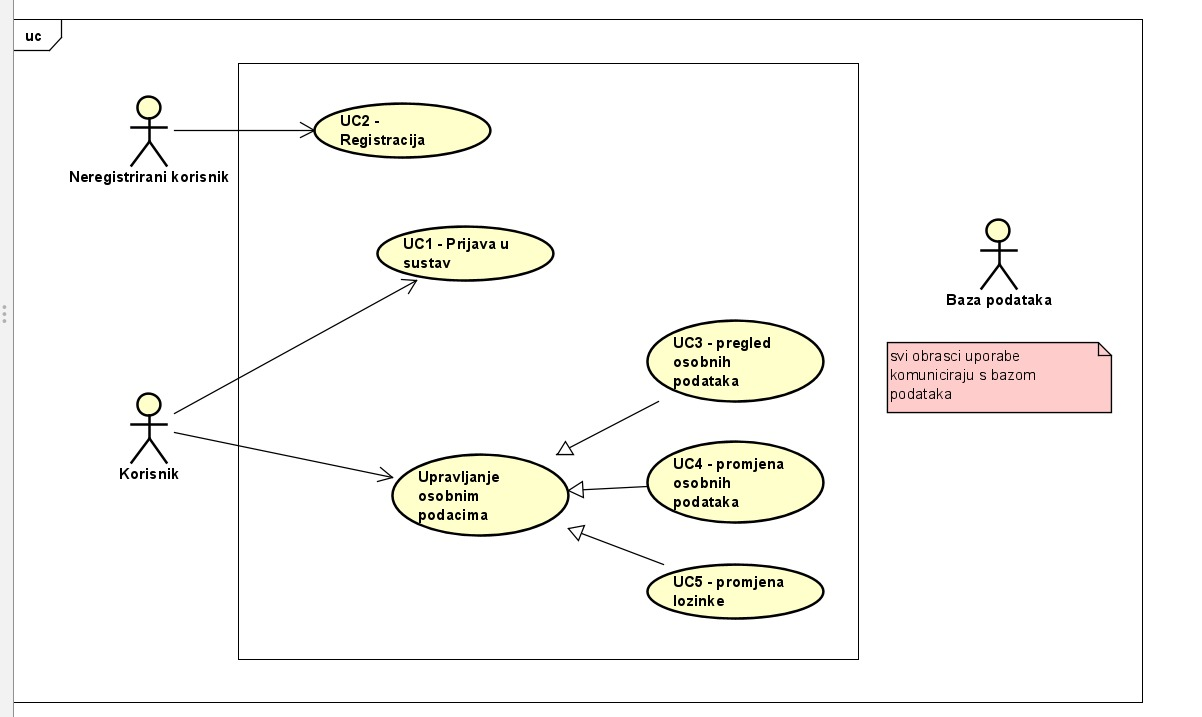
\includegraphics[scale=0.3]{slike/dijagram_obrasca_uporabe1.JPG} %veličina slike u odnosu na originalnu datoteku i pozicija slike
						\centering
						\caption{Dijagram obrasca uporabe - Korisnik i neregistrirani korisnik}
						\label{fig:dijagram_UC1}
					\end{figure}
					
					\begin{figure}[H]
						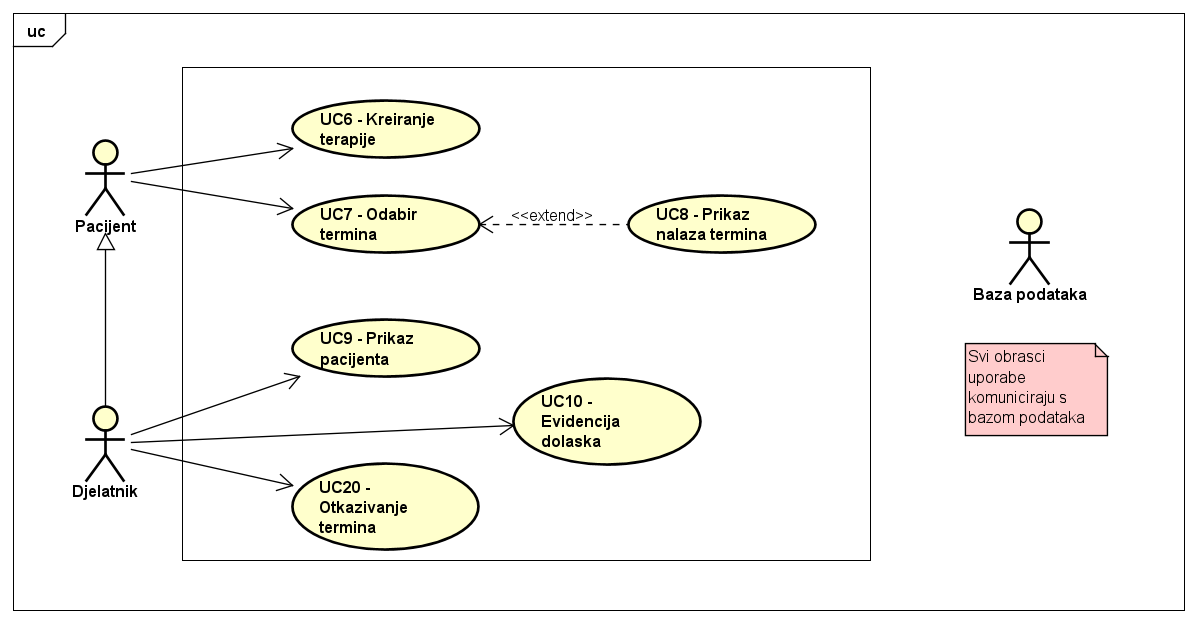
\includegraphics[scale=0.45]{slike/dijagram_obrasca_uporabe2.PNG} %veličina slike u odnosu na originalnu datoteku i pozicija slike
						\centering
						\caption{Dijagram obrasca uporabe - Djelatnik i pacijent}
						\label{fig:dijagram_UC2}
					\end{figure}
					
					\begin{figure}[H]
						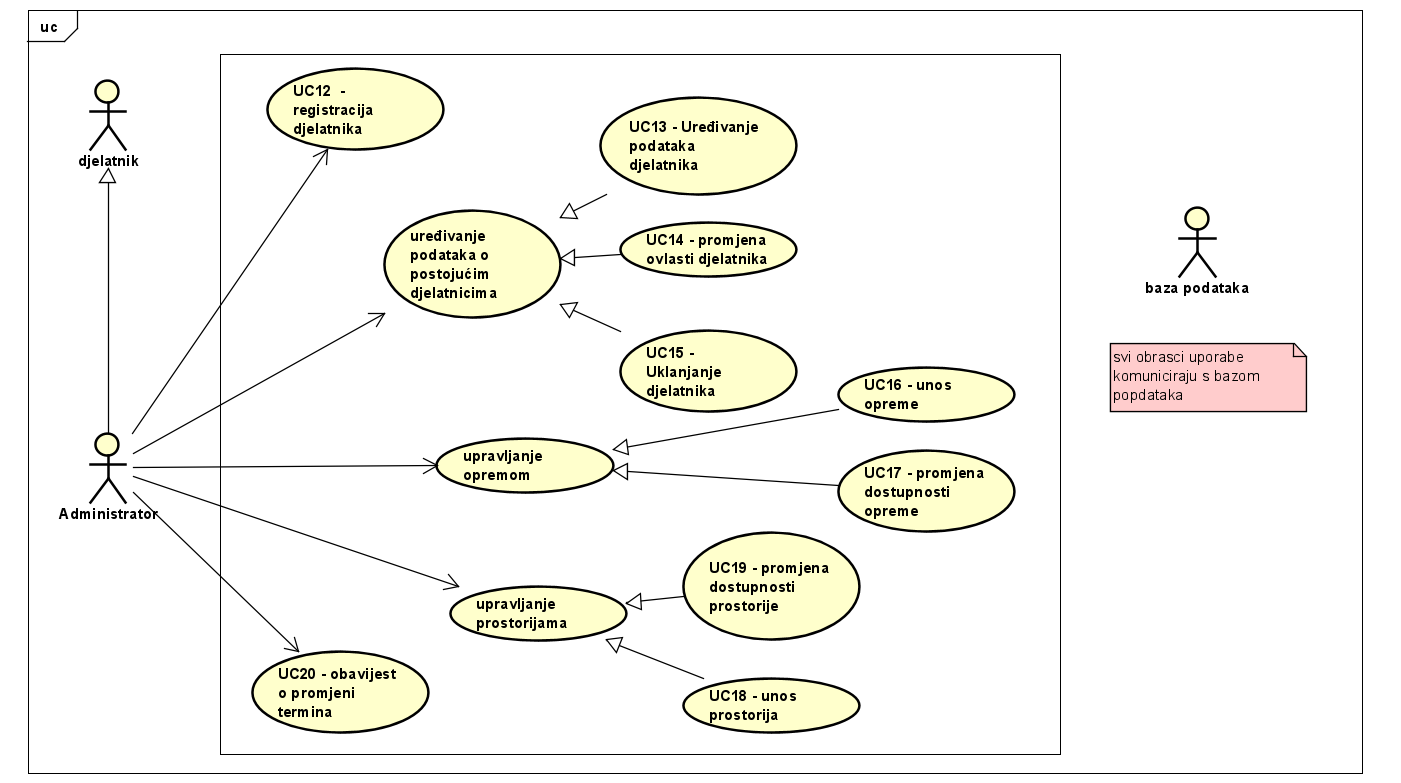
\includegraphics[scale=0.45]{slike/dijagram_obrasca_uporabe3.PNG} %veličina slike u odnosu na originalnu datoteku i pozicija slike
						\centering
						\caption{Dijagram obrasca uporabe - Administrator}
						\label{fig:dijagram_UC3}
					\end{figure}
					
				\eject		
				
			\subsection{Sekvencijski dijagrami}
				
				\textbf{\underbar{UC6 - Kreiranje terapije}}
				
				Pacijent šalje zahtjev poslužitelju za naručivanje na terapiju. Web aplikacija mu prikazuje obrazac koji mora ispuniti kako i se naručio na terapiju. Pacijent unosi potrebne podatke(ime i prezime liječnika koji ga je uputio na rehabilitaciju, vrstu terapije, opis oboljenja i zahtijevani postupak liječenja). Pacijent šalje popunjeni obrazac. Web aplikacija na temelju primljenih podataka provjerava kredibilitet liječnika u imeniku liječnika. Ovisno o rezultatu promjene web aplikacija, ako liječnik postoji u imeniku liječnika, sprema sve podatke u bazu podataka i prikazje stranicu za odabir termina. U slučaju da liječnik ne postoji u imeniku liječnika aplikacija ispisuje poruku "Liječnik ne postoji", pacijent u tom slučaju ponovno unosi to jest mijenja podatke i ponovno šalje obrazac. Pacijent može odustati od kreiranja terapije, pri čemu će mu se prikazati početna stranica.
				
				
				\begin{figure}[H]
					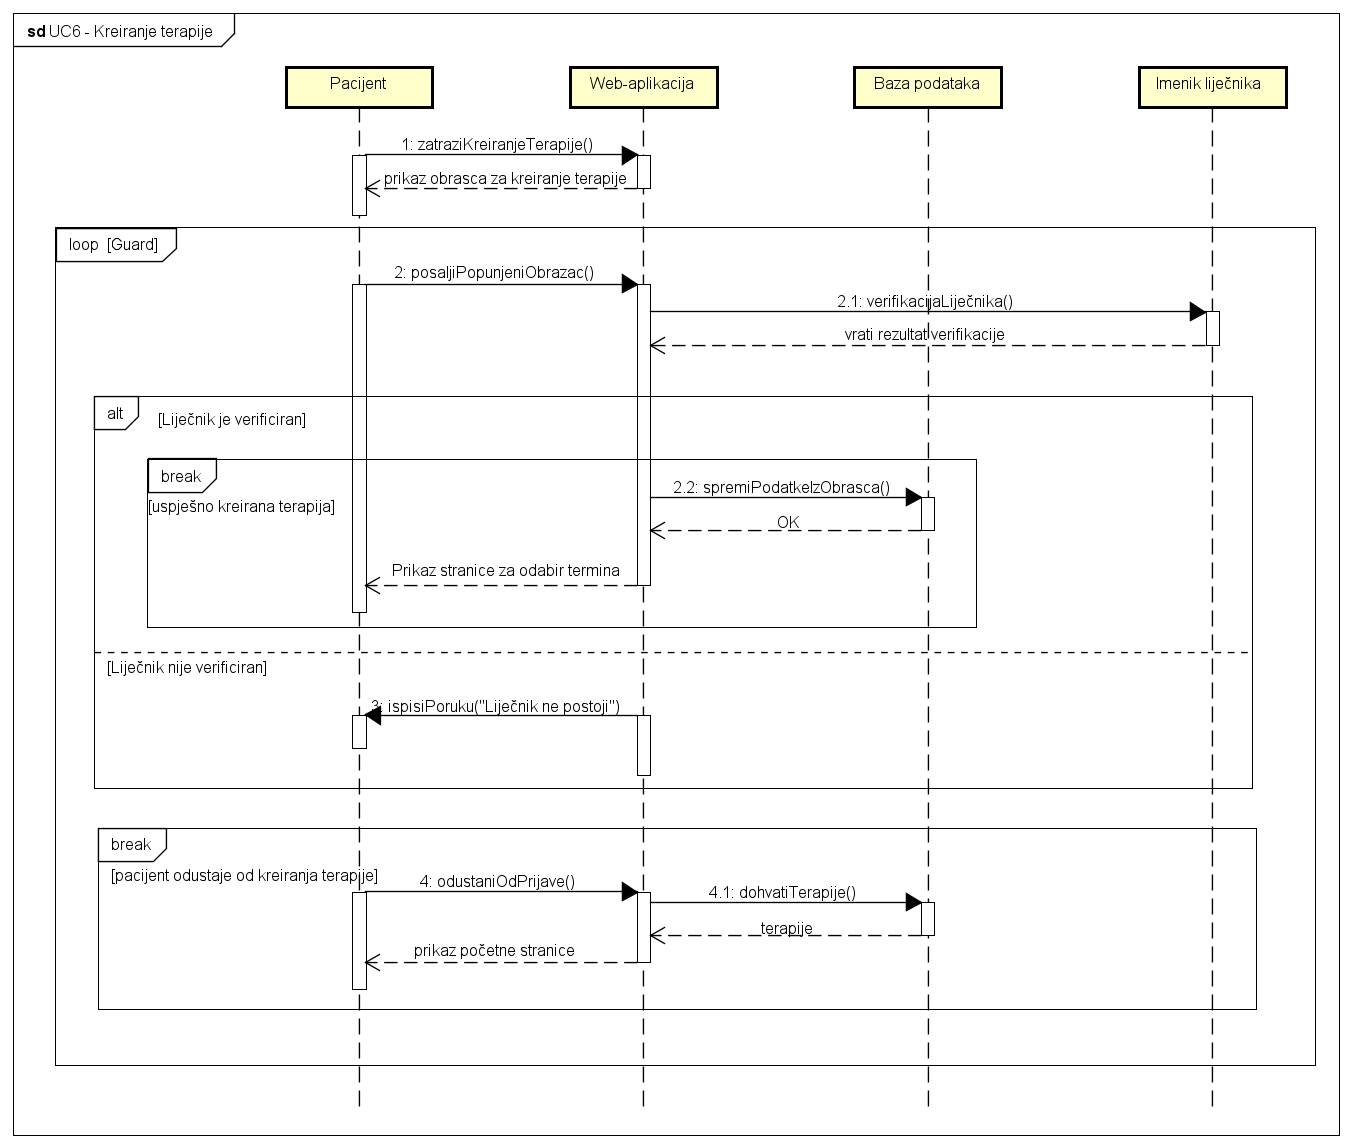
\includegraphics[scale=0.4]{slike/UC6_Kreiranje_terapije.PNG} %veličina slike u odnosu na originalnu datoteku i pozicija slike
					\centering
					\caption{Sekvencijski dijagram za UC6}
					\label{fig:sekvencijski_dijagram_1}
				\end{figure}
				
				\textbf{\underbar{UC10 - Evidencija dolaska}}
				
				Djelatnik odabire opciju evidentiraj pored termina odabranog pacijenta. Web aplikacija iz baze podataka dohvaća podatke o terapiji kojoj pripada odabrani termin, te nakon toga prikazuje obrazac za evidenciju s dohvaćenim podacima i prostorom za označavanje dolaska i unosom komentara. Djelatnik odabire status(odrađeno/ nije odrađeno) i piše komentar, nakon toga potvrđuje evidenciju i šalje popunjeni obrazac, web aplikacija potom unesene podatke sprema u bazu podataka izmjenjujući tako podatke o odabranom terminu. Nakon što su podaci uspješno uneseni web aplikacija traži od baze termine odabranog pacijenta i prikazuje stranicu s popisom termina tog pacijenta. U slučaju da je djelatnik odabrao krivi termin za evidenciju može odustati od evidentiranja, web aplikacija će dohvatiti podatke o terminima i prikazati stranicu s popisom termina odabranog pacijenta.
				
				\begin{figure}[H]
					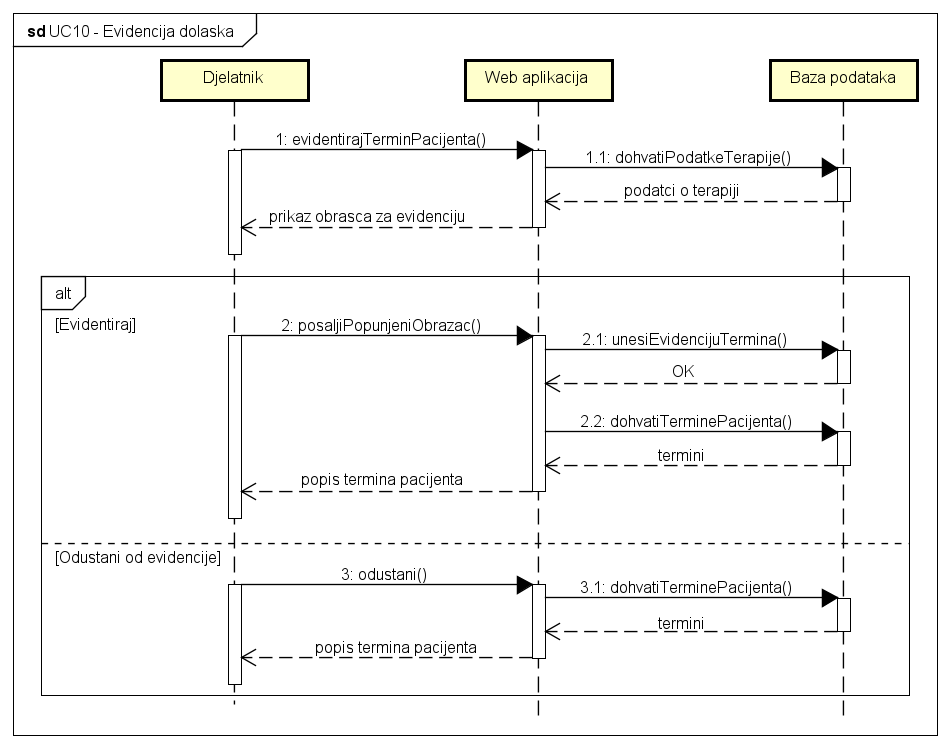
\includegraphics[scale=0.4]{slike/UC10_Evidencija_dolaska.PNG} %veličina slike u odnosu na originalnu datoteku i pozicija slike
					\centering
					\caption{Sekvencijski dijagram za UC10}
					\label{fig:sekvencijski_dijagram_2}
				\end{figure}
				
				
				\textbf{\underbar{UC19 - Obavijest o promjeni termina}}
				
				Administrator na svojoj stranici odabire opciju "Promjeni termin" te mu nakon toga web aplikacija otvara stranicu za promjenu termina. Administrator unosi pacijenta i pretražuje. Web aplikacija prima podatak i provjerava u bazi podataka ako pacijent postoji. Ako postoji web aplikacija odmah dohvaća neevidentirane termine odabranog pacijenta, te ih prikazuje administratoru. Administrator potom odabire termin koji želi promijeniti i web aplikacija mu pokazuje obrazac za dodjelu novog termina. Administrator unosi podatke o novom terminu (datum/soba/oprema) i aplikacija na temelju toga dohvaća moguće termine iz baze podataka. Administrator odabire neki od mogućih termina i opcionalno dodaje komentar. Nakon što administrator potvrdi odabrani termin web aplikacija dodaje termin u bazu podataka i šalje e-mail pacijentu s informacijama o promjeni termina, a administratoru se ponovno prikazuje stranica za promjenu termina. 
				
				U slučaju da pacijent kojeg je administrator unio ne postoji u bazi podataka aplikacija će ga obavijestiti o nepostojanju pacijenta. Administrator može ponovno unijeti pacijenta i ponoviti pretragu. 
				
				Administrator može odustati od promjene termina nakon čega mu se prikazuje početna stranica.
				
				\begin{figure}[H]
					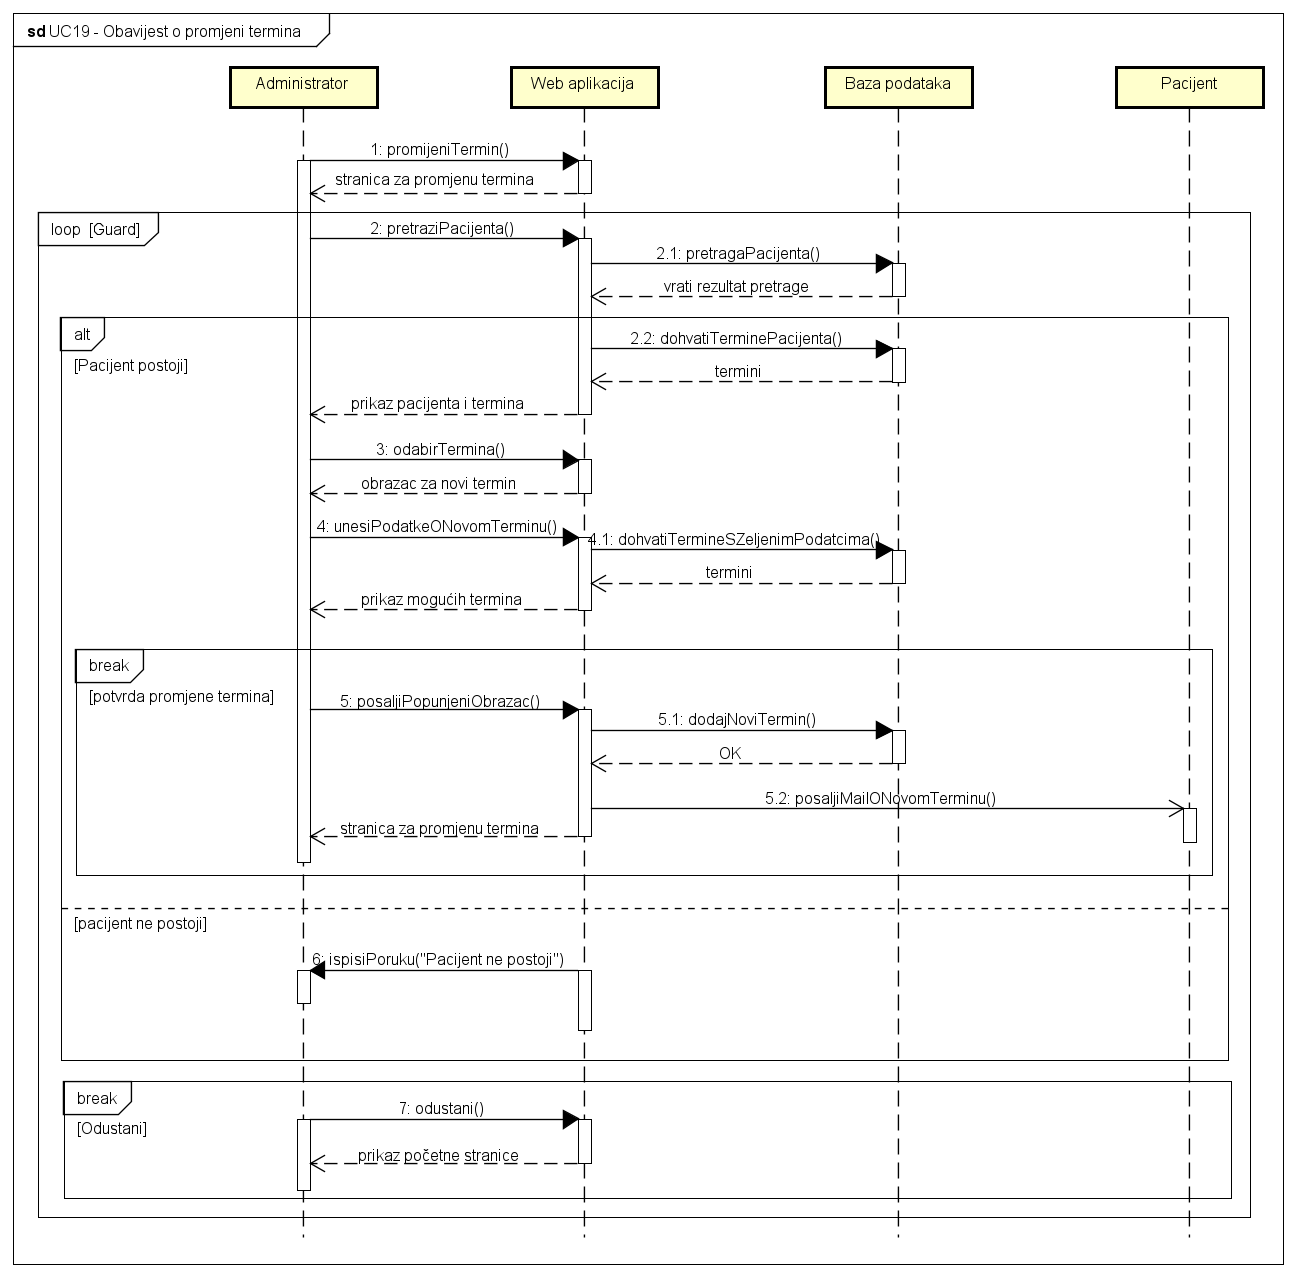
\includegraphics[scale=0.4]{slike/UC19_Obavijest_o_promjeni_termina.PNG} %veličina slike u odnosu na originalnu datoteku i pozicija slike
					\centering
					\caption{Sekvencijski dijagram za UC19}
					\label{fig:sekvencijski_dijagram_4}
				\end{figure}
				\eject
	
		\section{Ostali zahtjevi}
			 
			 \begin{packed_item}
			 	\item Sustav mora omogućiti istovremeni pristup više korisnika (100 korisnika istovremeno) uz očuvanje performansi.
			 	\item Poslužitelj mora vratiti odgovor na korisnički zahtjev unutar 5 sekundi.
<<<<<<<< HEAD
			 	\item Sustav mora biti dostupan korisnicima barem 99,99\% vremena unutar jedne godine.
=======
			 	\item Lozinka prije spremanja u bazu podataka mora biti kriptirana.
			 	\item Veza s bazom podataka mora biti brza i otporna na greške.
			 	\item Mora biti omogućen pristup sustavu iz javne mreže uz određenu razinu sigurnosti (HTTPS).
			 	\item Klijentska aplikacija mora raditi u pregledniku Google Chrome.
			 	\item Neispravno korištenje korisničkog sučelja ne smije narušiti funkcionalnost aplikacije.
			 	\item Korisničko sučelje mora podržavati hrvatski jezik.
			 	\item Korisničko sučelje mora biti jednostavno za upotrebu (intuitivno).
			 \end{packed_item}
			 
			 
			 
	